\documentclass[xcolor=dvipsnames]{beamer}
%\documentclass[usenames,dvipsnames]{beamer}
\usepackage[utf8]{inputenc}
\usepackage[T1]{fontenc}
\usepackage{tikz}
\usepackage{xytree}
\usepackage{comment}
\usepackage{multirow}
\usepackage{cancel}
\usepackage{colortbl}
\usepackage{tikz-qtree}
\usepackage{comment}

\usepackage{graphicx}
\usepackage{array}
%\usepackage{avm}
\usepackage{rotating}
\usepackage{amssymb}
\usepackage{makecell}
%\usepackage[british]{babel}
%\usepackage[utf8x,utf8]{inputenc}
\usepackage{xcolor}
\usepackage{enumitem}
\usepackage{eurosym}
\usepackage{hyperref}
\usepackage{comment}

\usepackage{xcolor}

%\newcommand{\ile}[1] {{\scriptsize \textcolor{RoyalBlue}{\textit{#1}}}}
%\newcommand{\lit}[1]{{\scriptsize \textcolor{RoyalBlue}{`#1'}}} %Literal translation
%\newcommand{\idio}[1]{{\scriptsize \textcolor{RoyalBlue}{`#1'}}}  %Idiomatic translation
%\newcommand{\exlit}[2]{\ile{#1}~\lit{#2}} %Example with a literal translation
%\newcommand{\exidio}[2]{\ile{#1}~\idio{#2}} %Example with an idiomatic translation
%\newcommand{\litidio}[2]{\lit{#1}$~\Rightarrow~$\idio{#2}} %Literal and idiomatic translation
%\newcommand{\exlitidio}[3]{\ile{#1}~\lit{#2}~$\Rightarrow$~\idio{#3}} %Example with a literal and a and idiomatic translation

\newcommand{\ana}[1] {{\scriptsize \textcolor{RoyalBlue}{#1}}} %Output of an analysis of a text 
\newcommand{\iletrue}[1] {\textcolor{OliveGreen}{#1}}
\newcommand{\ilefalse}[1] {\textcolor{Red}{#1}}
\newcommand{\ileunsure}[1] {\textcolor{BurntOrange}{#1}}
%\newcommand{\lex}[1] {\textbf{#1}} %Lexicalized component


%%%%%%%%%%%
%% in-line examples for languages in Latin script
%%%%%%%%%%
\usepackage{ulem}
\newcommand{\lex}[1]{\textbf{#1}}  %Lexicalized component
\newcommand{\litlex}[1]{\uwave{#1}}  %Literal reading of a lexicalized component
\newcommand{\coinlex}[1]{\dashuline{#1}}  %Coincindental co-occurrence of lexicalized components

\newcommand{\ile}[1]{\textcolor{blue}{\textsl{#1}}} %In-line example  
\newcommand{\lit}[1]{\textcolor{gray}{(lit. '\textit{#1}')}} %Literal translation
\newcommand{\idio}[1]{\textcolor{brown}{`#1'}}  %Idiomatic translation
\newcommand{\exlit}[2]{\ile{#1}~\lit{#2}} %Example with a literal translation
\newcommand{\exidio}[2]{\ile{#1}~\idio{#2}} %Example with an idiomatic translation
\newcommand{\litidio}[2]{\lit{#1}~\idio{#2}} %Literal and idiomatic translation
\newcommand{\exlitidio}[3]{\ile{#1}~\lit{#2}~\idio{#3}} %Example with a literal and a and idiomatic translation


%%%%%%%%%%
\setbeamertemplate{itemize/enumerate subbody begin}{\scriptsize}

\usepackage{relsize}
\newcommand{\lang}[1]{\textcolor{gray}{\textsmaller[1.5]{\fbox{\textsf{#1}}}}}

\newcommand{\formatPOS}[1]{{\scriptsize #1}}
\newcommand{\formatMorph}[1]{\_}  %{{\tiny #1}}
\newcommand{\formatMWE}[1]{\textcolor{blue}{#1}}

\newcommand*\GBitem{%
   \item[{
\includegraphics[width=0.2cm]{Images/Flags/UnitedKingdom.png}}]}
\newcommand*\FRitem{%
   \item[{
\includegraphics[width=0.2cm]{Images/Flags/France.png}}]}
\newcommand*\PLitem{%
   \item[{\includegraphics[width=0.2cm]{Images/Flags/Poland.png}}]}
\newcommand*\SRitem{%
   \item[{\includegraphics[width=0.2cm]{Images/Flags/Serbia.png}}]}
\newcommand*\ITitem{%
   \item[{\includegraphics[width=0.2cm]{Images/Flags/Italy.png}}]}

\newcommand{\gloss}[1] {
  {\scriptsize \textcolor{blue}{'#1'}}}

%%%%% Linguistic examples in blue scriptsize italic
\newcommand{\exa}[1]{\textcolor{blue}{\textit{#1}}}

%%%%% Bibliographic references in scriptsize
\newcommand{\mycite}[1]{{\scriptsize \textcolor{magenta}{\cite{#1}}}}
\newcommand{\minicite}[1]{{\scriptsize \cite{#1}}}
%\newcommand{\minicitet}[1]{{\scriptsize \citet{#1}}}

%%%%% Bets results
\newcommand{\best}[1]{\textbf{#1}}



\usetheme{Darmstadt}
\setbeamertemplate{footline}
{
  \leavevmode%
  \hbox{%
  \begin{beamercolorbox}[wd=.333333\paperwidth,ht=2.25ex,dp=1ex,center]{author in head/foot}%
    \usebeamerfont{author in head/foot}\insertshortauthor%~~\beamer@ifempty{\insertshortinstitute}{}{(\insertshortinstitute)}
  \end{beamercolorbox}%
  \begin{beamercolorbox}[wd=.333333\paperwidth,ht=2.25ex,dp=1ex,center]{title in head/foot}%
    \usebeamerfont{title in head/foot}\insertshorttitle
  \end{beamercolorbox}%
  \begin{beamercolorbox}[wd=.333333\paperwidth,ht=2.25ex,dp=1ex,right]{date in head/foot}%
    \usebeamerfont{date in head/foot}\insertshortdate{}
    \hspace*{2em}
    \insertframenumber{} / \inserttotalframenumber\hspace*{2ex} 
  \end{beamercolorbox}}%
  \vskip0pt%
}
\setbeamertemplate{navigation symbols}{}
\beamertemplatenavigationsymbolsempty


%\usecolortheme[RGB={0,100,100}]{structure}
%\usecolortheme[named=BrickRed]{structure}

\setbeamerfont{author}{size=\large}
\setbeamerfont{title}{series=\bfseries,size=\LARGE}
%%%%%%%%%%%%%%%%%%%%%%%%%%%%%%%%%%%%%%%%%%%%%%%%%%%%%%%%%%%%%%%%%%%%%%%%
%\usecolortheme{crane}
\usecolortheme{seagull}

\setlist{labelindent=1em,leftmargin=1em}
\setitemize{label=\usebeamerfont*{itemize item}%
  \usebeamercolor[fg]{itemize item}
  \usebeamertemplate{itemize item}}




%%%%%%%%%%%%%%%%%%%%%%%%%%%%%%%%%%%%%%%%%%%%%%%%%%%%%%%%%%%%%%%%%%%%%%%%%%%%%%%%%%%%

\title[PARSEME Intro]{Introduction to annotating verbal multiword expressions in the PARSEME framework\\
\includegraphics[scale=0.3]{Images/parseme-logo.png}}

\author{Carlos Ramisch, Agata Savary}

\institute[shortinst]{Aix-Marseille Université, Université Paris-Saclay, France}



\date[UniDive, 19/06/2023]{UniDive webinar, 19 June 2023}

\begin{document}

%\frame{\titlepage}
\begin{frame}

\titlepage
%\textgreek{καλημέρα & καλωσήρθατε στην}
\end{frame}

%%%%%%%%%%%%%%%%%%%%%%%%%%%%%%%%%%%%%%%%%%%%
\section{PARSEME} 
\subsection{}

%%%%%%%%%%%%%
\begin{frame}
  \frametitle{PARSEME}
  
\begin{scriptsize}
  
\begin{block}{Network}
\begin{itemize}
\item COST Action on \textbf{Parsing and Multiword Expressions} (MWEs) funded by European Commission in \textbf{2013-2017}, still \textbf{active}
\item 31 countries, 30 languages and 6 dialects from 10 language genera
\item Outcomes: publications, resources, tutorials, methodologies, PMWE book series 
\end{itemize}
\end{block}

\begin{block}{MWE corpora (\textcolor{magenta}{\url{https://gitlab.com/parseme/corpora/-/wikis/}})}
\begin{itemize}
\item \textbf{Collaborative} effort: 25 language teams, 31 language leaders, 160 annotators
\item Annotation \textbf{guidelines} for \textbf{verbal} MWEs \textbf{unified} across some 25 languages
\item Corpora \textbf{manually} annotated for MWEs: \textbf{25 languages}, open licenses
\item \textbf{Continuous enhancements} of the guidelines and corpora
\end{itemize}
\end{block}

\end{scriptsize}

\begin{tikzpicture}[remember picture,overlay]
\node at (8.5,6.8) {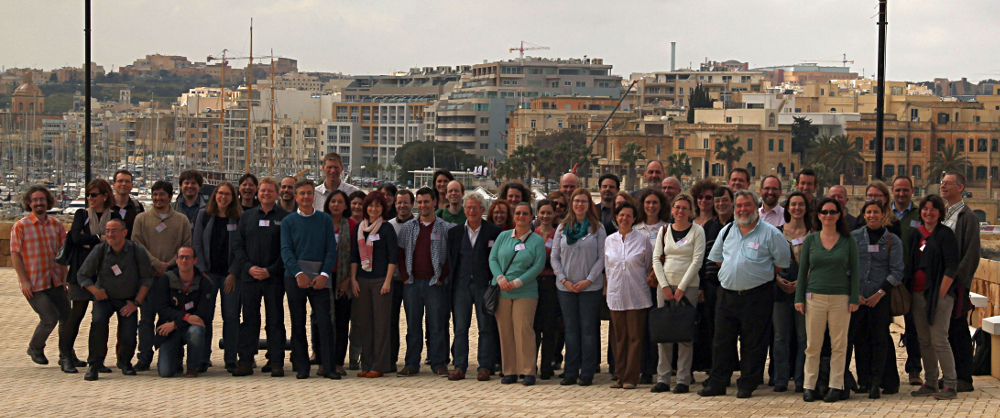
\includegraphics[scale=0.15]{Images/parseme-malta.jpg}};
\end{tikzpicture}

\end{frame}

%%%%%%%%%%%%%%%%%%%%%%%%%%%%%%%%%%%%%%%%%%%
\section{MWEs} 
\subsection{}

%%%%%%%%%%%%%
\begin{frame}
  \frametitle{Multiword expressions}

\begin{block}{}
\textit{The \textcolor{red}{\textbf{prime time}} speech by \textcolor{blue}{\textbf{first lady}} \textcolor{green}{\textbf{Michelle Obama}} \textcolor{magenta}{\textbf{set}} the house \textcolor{magenta}{\textbf{on fire}}. She made \textcolor{brown}{\textbf{crystal clear}} which issues she \textcolor{violet}{\textbf{took to heart}} but she was \textcolor{orange}{\textbf{preaching to the choir}}.}
\end{block}

\begin{block}{Definition \cite{baldwin-kim:2010:handbook}}
Combination of at least \textbf{two words} which exhibits lexical, morphological, syntactic, semantic and /or statistical \textbf{idiosyncrasies}.
\end{block}

\begin{block}{Idiosyncrasy}
A mode of behaviour or a property which is \textbf{particular} to an (few) individual(s). An \textbf{unusual} feature.
\end{block}


\end{frame}

%%%%%%%%%%%%%

\begin{frame}
  \frametitle{Sample idiosyncrasies in MWEs}

\begin{scriptsize}

\begin{block}{}%Major types  of idiosyncrasies in MWEs}
   \begin{itemize}
   \item \textbf{Non-compositional semantics}: the meaning of a MWE is surprising, given the meanings of its component words
      \begin{itemize}
      %\GBitem 
      \item[]\lang{EN} \exidio{to \lex{pull} one's \lex{leg}}{to tease someone playfully}
      %\ITitem 
      \item[]\lang{IT} \exlitidio{\lex{lasciar perdere}}{to let lose}{to give up}
      \end{itemize}
   \item Morphosyntactic \textbf{irregularity} (token\footnote{{\scriptsize Token = individual occurrence}}-specific):
      \begin{itemize}
      %\FRitem 
      \item[]\lang{FR} \exidio{\lex{grand-mères}}{grand$_{sing.masc}$-mothers$_{pl.fem}$} (defective agreement)
      %\GBitem 
      \item[]\lang{EN} \exidio{\lex{by and large}}{mostly} (Prep Conj Adj is an irregular syntactic structure)
      %\GBitem 
      \item[]\lang{EN} \exidio{to \lex{go nuts}}{to get crazy} (\ile{go} alone is intransitive)
      \end{itemize}
   \item Restricted morphosyntactic \textbf{flexibility} (type\footnote{{\scriptsize Type = sets of surface realizations of the same expression}}-specific):
      \begin{itemize}
      %\GBitem 
      \item[]\lang{EN} \exidio{\lex{the die is cast}}{a point of no-retreat has been passed} vs. \ile{\#someone cast the die}
      \end{itemize}
   \end{itemize}
\end{block}

\end{scriptsize}

\end{frame}


%%%%%%%%%%%%%%%
\begin{frame} 
\frametitle{Restricted flexibility: a proxy for semantic non-compositionality}

\begin{block}{}
A MWE is (much) \textbf{less flexible} (variable) than a regular construction of the same syntactic structure.
\end{block}

\vspace{0.5cm}

\begin{scriptsize}
\centering
\setlength{\tabcolsep}{0.5mm}
\begin{tabular}{|l|p{5.4cm}|p{1.8cm}|}\hline
\textbf{Regular construction} & \textbf{MWE} & \begin{tabular}{l}\textbf{MWE}\\\textbf{property}\end{tabular} \\\hline\hline

  \begin{tabular}{l}\ile{warm soup} $\approx$\footnote{{\tiny '$\approx$' means that the meaning shift is predictable from the formal change}} \ile{hot soup} $\approx$ \\ \ile{warm stew}\end{tabular}
& \begin{tabular}{l}\ile{\lex{hot dog}} vs. \ile{\#warm dog} vs. \ile{\#hot terrier}\end{tabular}
& \begin{tabular}{l}Lexical\\inflexibility\end{tabular} \\\hline

  \begin{tabular}{l}\ile{to throw meat to the lions} $\approx$ \\ \ile{to throw meat to the \underline{lion}}\end{tabular}
& \begin{tabular}{l}\ile{to \lex{throw} someone \lex{to the lions}} vs. \\ \ile{\#to throw someone to the \underline{lion}}\end{tabular}
& \begin{tabular}{l}Morphological\\inflexibility\end{tabular} \\\hline

  \begin{tabular}{l}\ile{the die is stolen} $\approx$ \\ \ile{\underline{someone stole} the die}\end{tabular}
& \begin{tabular}{l}\ile{\lex{the die is cast}} vs. \\ \ile{\#\underline{someone cast} the die}\end{tabular} 
& \begin{tabular}{l}Syntactic\\inflexibility\end{tabular} \\\hline

\end{tabular}
\end{scriptsize}

\end{frame}

%%%%%%%%%%%%%%%%
\begin{frame} 
\frametitle{Focus on \textbf{verbal} MWEs -- challenges}

\begin{scriptsize}
\begin{itemize}
\item Discontinuity:
	\begin{itemize}
	\item[] \lang{EN} \ile{Trying hard to \textbf{bear} all these more or less important indications \textbf{in mind}}
	\item[] \lang{DE} \ile{Klaus Kinkel (FDP) \textbf{ging} in seiner Würdigung des Mauerfalls zumindest auf den 9. November 1938 \textbf{ein}.}
    	\end{itemize}
\item Flexibility: morphological, syntactic, lexical
	\begin{itemize}
	\item[] \lang{EN} \ile{he \lex{broke} my \lex{fall}} vs.~\ile{both of my \lex{falls} were hard to \lex{break}}
	\end{itemize}
\item Ambiguity: idiomatic vs.~literal readings
	\begin{itemize}
	\item[] \lang{EN} \exidio{she \lex{takes the cake}}{she is the most outstanding} vs. \ile{she takes the cake}
	\end{itemize}
\item Overlaps:
   	\begin{itemize}
	\item[] \lang{EN} \ile{\underline{\lex{take}} a \lex{walk} and then a long \lex{shower}} (coordination)
	\item[] \lang{EN} \ile{\lex{take} the fact that I \underline{\lex{gave up}} \lex{into account}} (interleaving)
	\item[] \lang{EN} \ile{\lex{\underline{let} the cat \underline{out} of the bag}} (nesting)
	\end{itemize}
\item Multiword tokens
	\begin{itemize}
	\item[] \lang{ES}  \exlitidio{\lex{abstener}|\lex{se}}{abstain oneself}{abstain} vs. \ile{me abstengo}
	\item[] \lang{DE}  \exlitidio{\lex{auf}|\lex{machen}}{out|make}{open} vs. \ile{macht auf}
	\end{itemize}
\item Different languages $\Rightarrow$ different behavior, linguistic traditions\ldots
\end{itemize}
\end{scriptsize}

\end{frame}

%%%%%%%%%%%%%%%%
\begin{frame} 
\frametitle{Neutralizing flexibility}

\begin{block}{Canonical form}
Least syntactically marked syntactic variant which preserves the idiomatic reading (active voice is less marked then passive, etc.)

\begin{tabular}{ccc}
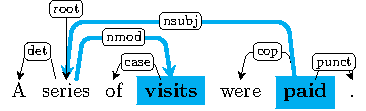
\includegraphics[width=.45\textwidth]{Images/series-of-visits-paid} & 
$\Longrightarrow$ &
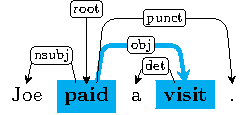
\includegraphics[width=.25\textwidth]{Images/pay-visit}
\end{tabular}

\end{block}

\begin{block}{}
Canonical forms are useful for \textbf{formalizing} the morpho-syntactic properties of MWEs. This is useful e.g. for \textbf{annotation guidelines}.
\end{block}

\end{frame}

%%%%%%%%%%%%%%%%
\begin{frame} 
\frametitle{Focus on \textbf{verbal} MWEs}

\begin{scriptsize}

%\vspace{-0.2cm}
\begin{block}{Verbal MWEs (VMWEs)}
MWEs whose \textbf{canonical form} is such that:
    \begin{itemize}
    \item its syntactic head is a verb V 
    \item its other lexicalized components form phrases directly dependent on V, i.e. the \textbf{dependency subgraph} of the lexicalized components is weakly \textbf{connected}
    \end{itemize}

\begin{tabular}{cc}
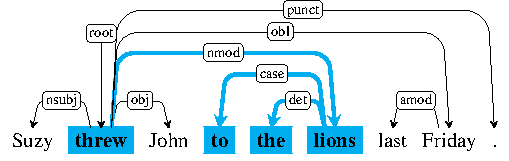
\includegraphics[width=.55\textwidth]{Images/throw-to-the-lions} &
\xcancel{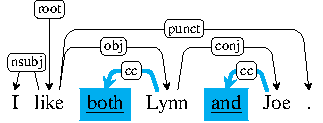
\includegraphics[width=.35\textwidth]{Images/both-and}}
\end{tabular}

\end{block}

\end{scriptsize}

\end{frame}


\begin{comment}
\end{comment}

%%%%%%%%%%%%%%%%%%%%%%%%%%%%%%%%%%%%%%%%%%%
\section{Annotation} 
\subsection{}

%%%%%%%%%%%%%%%%
\begin{frame} 
\frametitle{Annotating MWEs in a corpus}

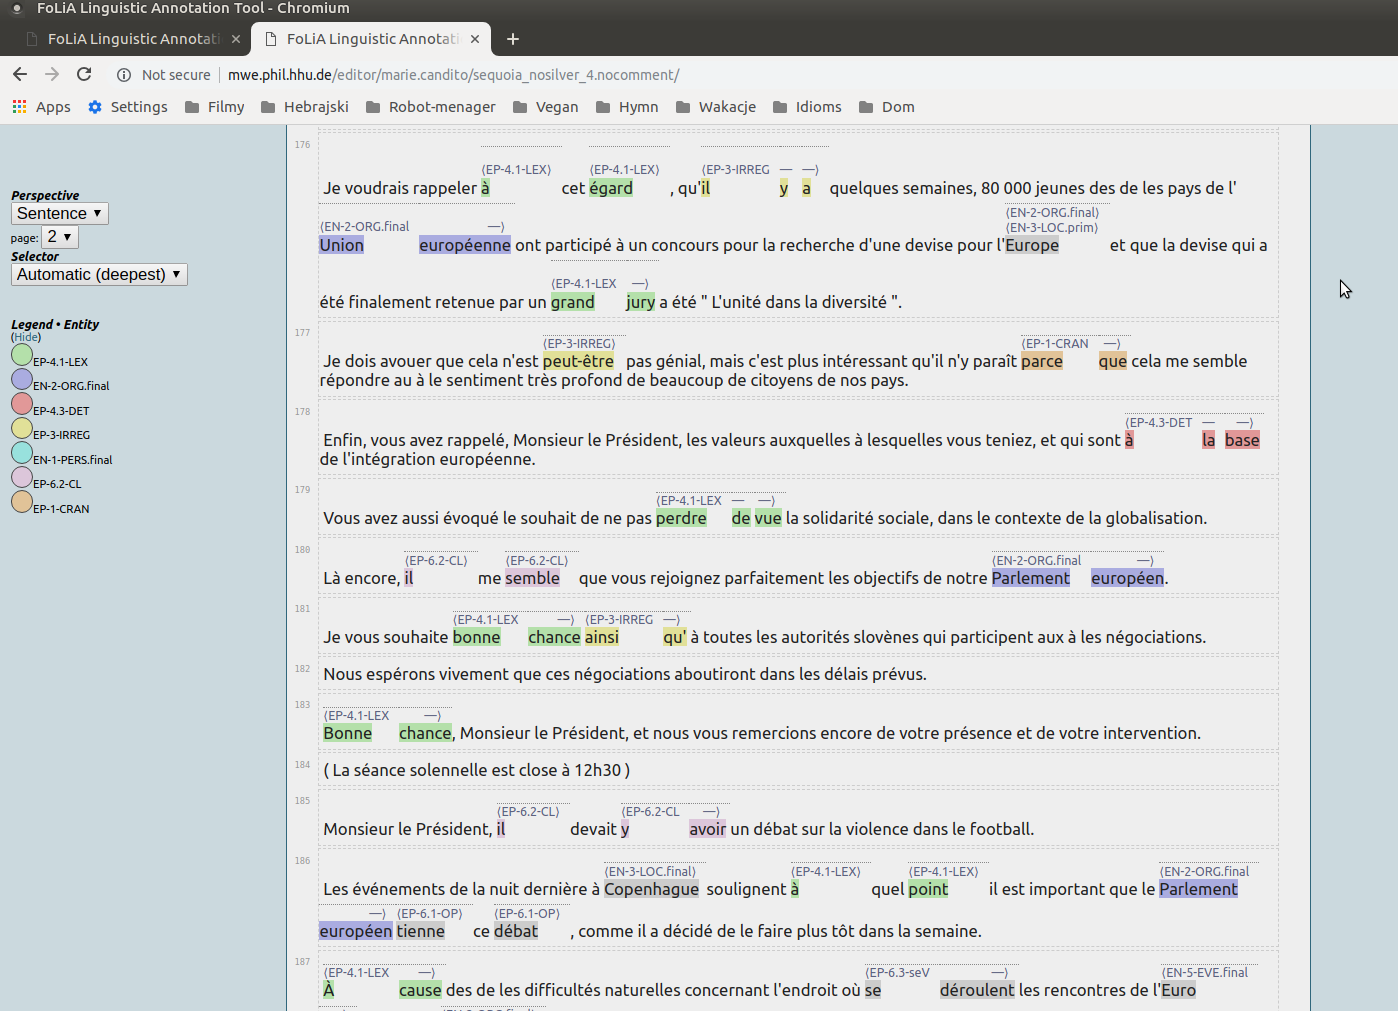
\includegraphics[scale=0.23]{Images/flat.png}

\end{frame}

%%%%%%%%%%%%%
\begin{frame}
  \frametitle{PARSEME annotation guidelines \textcolor{magenta}{{\scriptsize (\url{https://parsemefr.lis-lab.fr/parseme-st-guidelines/1.2})}}}

\begin{scriptsize}

\vspace{-0.2cm}

\begin{block}{Objectives} 
\begin{itemize}
\item Formalise idiomaticity in a \textbf{cross-linguistically unified} and \textbf{computationally tractable} way
\item Unify what is truly \textbf{similar}, emphasise what is \textbf{language-specific}
\item Make the annotation \textbf{reproducible}
\end{itemize}
\end{block}

\vspace{-0.2cm}

\begin{block}{Principles and constraints} 
\begin{itemize}
\item Annotation follows a \textbf{decision diagram} (unique starting point)
\item Non-compositionality is a matter of \textbf{scale} but decisions must be \textbf{binary}
\item \textbf{Semantic non-compositionality} is the major property to capture but is \textbf{hard to test directly}
\item Lexical and morpho-syntactic \textbf{inflexibility} is considered a \textbf{proxy} for semantic non-compositionality
\item Inflexibility tests are driven by the \textbf{syntactic structure}
\item Strong dependence on the underlying \textbf{syntactic theory}
\item PARSEME annotation largely \textbf{relies on the UD} annotation of morpho-syntax
\end{itemize}
\end{block}

\end{scriptsize}

\end{frame}



%%%%%%%%%%%%%%%%%%%%%%%
\begin{frame}
  \vspace*{-5pt}
  \frametitle{VMWE typology (v. 1.2)}

\begin{scriptsize}
\begin{block}{}
\begin{itemize}
\item \textbf{Universal} categories (valid for all languages):
   \begin{itemize}
   \item light verb constructions (\textbf{LVCs})
	\begin{itemize}
	\item \textbf{LVC.full}: \lang{EN} \ile{to \lex{give} a \lex{lecture}}
	\item \textbf{LVC.cause}: \lang{EN} \ile{to \lex{grant} \lex{rights}}
	\end{itemize}
   \item verbal idioms (\textbf{VIDs})
	\begin{itemize}
	\item[] \lang{EN} \ile{to \lex{call it a day}}
	\end{itemize}
   \end{itemize}
\item \textbf{Quasi-universal} categories (valid for many languages):
   \begin{itemize}
   \item inherently reflexive verbs (\textbf{IRVs})
	\begin{itemize}
	\item[] \lang{FR} \exidio{\textcolor{RoyalBlue}{\lex{s'évanouir}}}{to faint}
	\end{itemize}
   \item verb-particle constructions (\textbf{VPCs})
	\begin{itemize}
	\item \textbf{VPC.full} \lang{EN} \exidio{to \lex{do in}}{to kill}
	\item \textbf{VPC.semi} \lang{EN} \exidio{to \lex{eat up}}{to eat completely}
	\end{itemize}
   \item multi-verb constructions (\textbf{MVCs})
	\begin{itemize}
	\item[] \lang{HI} \exlitidio{\textcolor{BlueViolet}{\lex{kar le-na}}}{do take.INF}{to do something (for one's own benefit)}
	\end{itemize}
   \end{itemize}
\item \textbf{Experimental} (optional) category
   \begin{itemize}
   \item inherently adpositional verbs (\textbf{IAVs})
	\begin{itemize}
	\item[] \lang{EN} \ile{to \lex{come across} sth/sb}, \ile{to \lex{rely on} sth/sb}
	\end{itemize}	
   \end{itemize}
\end{itemize}
\end{block}
\end{scriptsize}

\end{frame}

%%%%%%%%%%%%%%%%
\begin{frame} 
\frametitle{Unified multilingual annotation guidelines \href{http://parsemefr.lif.univ-mrs.fr/parseme-st-guidelines/1.1}{\beamergotobutton{[link]}}}

\ile{the fate of the republic rests on your shoulders}

\begin{scriptsize}
\begin{block}{Annotation exercise}
\begin{itemize}
\item Step 1: identify the candidate and its canonical form: \ile{rests on your shoulders}
\item Step 2: determine the lexicalized components
   \begin{itemize}
   \item \ile{\lex{rests on} your/our \lex{shoulders}}, \ile{\lex{rests on} the \lex{shoulders} of the deputies}, etc.
   \end{itemize}
\item Follow the \href{http://parsemefr.lif.univ-mrs.fr/parseme-st-guidelines/1.1/?page=040\_Annotation\_process\_-\_decision\_tree}{\beamergotobutton{decision tree}}
   \begin{itemize}
   \item S.1 [1HEAD] (YES): \ile{rests} is the only verbal head of the whole phrase
   \item S.2 [1DEP] (YES): \ile{on shoulders} is the only lexicalized dependent of \ile{rests}
   \item S.3 [LEX-SUBJ] (NO): \ile{on} shoulders is not the subject of \ile{rests}
   \item S.4 [CATEG] (extended NP): \ile{on shoulders} is a prepositional phrase
   \item LVC.0 [N-ABS] (NO): \ile{shoulders} is not abstract
   \item VID.1 [CRAN] (NO): all components function also as stand-alone words
   \item VID.2 [LEX] (YES): \#\ile{remains on your shoulders}, \#\ile{rests on your back/arms/head}
   \end{itemize}
\item Outcome: \textbf{VID}
\end{itemize}
\end{block}

\end{scriptsize}

\end{frame}


%%%%%%%%%%%%%%%%%%%%%%%%%%%%%%%%%%%%%%%%%%
\section{Conclusions}  
\subsection{}

%%%%%%%%%%%%%%%%%%%%%%%
\begin{frame}
   \frametitle{Conclusions}

\begin{scriptsize}
\begin{block}{Results}
\begin{itemize}
\item \textbf{Strong progress} on automatic identification of verbal MWEs (resources \& tools)
\item MWE identification is more challenging than related tasks (e.g. NER)
\item \textbf{Unseen} data are critically hard
\item Much progress can be gained from careful \textbf{account of variability} of seen VMWEs
\item Contextual \textbf{embeddings} help generalize over (the few) \textbf{lexically flexible} VMWEs
\item \textbf{Few} efforts on coupling supervised with \textbf{unsupervised} methods
\item Truly \textbf{unseen idioms} cannot be found
\item Zipfian tail still seems long (diversity is weak)
\end{itemize}
\end{block}

\begin{block}{Position statement}
\begin{itemize}
\item The difficulties of MWE identification lie in the very \textbf{nature of MWEs}
\item \textbf{Lexicons} balance the Zipfian tail on syntactically diverse and figurative idioms
\item MWE identification should be coupled with MWE \textbf{lexicons and discovery tools}
\item \textbf{Computationally less intensive} methods should be developed
\item Lexical \textbf{diversity} should be preserved
\end{itemize}
\end{block}

\end{scriptsize}

\end{frame}


%%%%%%%%%%%%%%%%%%%%%%%
\setbeamertemplate{footline}{}
\newcounter{finalframe}
\setcounter{finalframe}{\value{framenumber}}
%%%%%%%%%%%%%%%%%%%%%%%

%%%%%%%%%%%%%%%%%%%%%%%
%\begin{frame}
%   \frametitle{The Holy Grail}

%\end{frame}

%%%%%%%%%%%%%%%%%%%%%%%%%%%%%%

\setcounter{framenumber}{\value{finalframe}}
%%%%%%%%%%%%%%%%
\section{Bibliography} %and Motivation
\subsection{}
%%%%%%%%%%%%%%%%

\scriptsize{\bibliographystyle{natbib-compact}}
%\scriptsize{\bibliographystyle{plainnat}}

\begin{frame}[allowframebreaks]
\frametitle{Bibliography}

\tiny{\bibliography{biblio}}

\end{frame}

%%%%%%%%%%%%%%%%%%%%%%%%%%%%%%
\setcounter{framenumber}{\value{finalframe}}
%%%%%%%%%%%%%%%%%%%%%%%%%%%%%%

%%%%%%%%%%%%%%%%
%\section{IAA} %and Motivation
%\subsection{}

%%%%%%%%%%%%%%%%%%%%%%%
\begin{frame}
  \vspace*{-5pt}
  \frametitle{Inter-annotator agreement}


\begin{block}{What is IAA?}
A measure meant to assess:
\begin{itemize}
\item hardness of the annotation task
\item quality of the annotation methodology
\item quality of the resulting annotations
\end{itemize}
\end{block}

\begin{block}{Popular IAA measure: Cohen's $\kappa$}
\begin{itemize}
\item Setting: two raters classify \textbf{N items} into C \textbf{mutually exclusive categories}
\item Measure: \\
~~~~~~~~~~$\kappa = \frac{P_O - P_E}{1-P_E}$
   \begin{itemize}
   \item $P_O$ - observed agreement
   \item $P_E$ - expected (chance) agreement
   \end{itemize}
\end{itemize}
\end{block}

\end{frame}

%%%%%%%%%%%%%%%%%%%%%%%
\begin{frame}[label={iaa}]
  \vspace*{-5pt}
  \frametitle{Challenges for IAA}

\begin{scriptsize}

\begin{block}{Challenges features of VMWE annotation}
\begin{itemize}
\item \emph{Unitising}, i.e.\ identifying the boundaries of a VMWE in the text
\item \emph{Categorisation}, i.e.\ assigning each identified VMWE to one of the pre-defined categories
\item \emph{Sporadicity}, i.e.\ the fact that not all text tokens are subject to annotation (unlike in part-of-speech annotation, for instance);
\item \emph{Free overlap}, e.g.\ in (CS) \exidio{\lex{ukládal} různé \lex{sankce} a \lex{penále}}{put various sanctions and penalties}, where two LVCs share a light verb;
\end{itemize}
\end{block}

\begin{block}{Challenges for IAA}
\begin{itemize}
\item What are the atomic units (Cohen's items) of annotation?
   \begin{itemize}
   \item text \textbf{tokens} $\Rightarrow$ categories are not mutually exclusive due to ovelaps
   \item text \textbf{spans} $\Rightarrow$ two annotators may end up with different sets of units $\Rightarrow$ unitising is part of the IAA measure
   \end{itemize}
\item In unitising IAA: What is the chance agreement?
\end{itemize}
\end{block}

\end{scriptsize}

\end{frame}


%%%%%%%%%%%%%%%%%%%%%%%
\begin{frame}[label={iaa}]
  \vspace*{-5pt}
  \frametitle{Three IAA measures in the PARSEME corpus}

%\begin{scriptsize}

\begin{block}{$F_{span}$}
\begin{itemize}
\item F-measure of annotator A1 prediction wrt. A2 (MWE-based or token-based)
\end{itemize}
\end{block}

\begin{block}{$\kappa_{span}$}
\begin{itemize}
\item Task simplification: For each verb $v$, decide if $v$ belongs to a VMWE or not.
\item Cohen's $\kappa$ in which the chance agreement is based on the number of verbs
\end{itemize}
\end{block}

\begin{block}{$\kappa_{cat}$}
\begin{itemize}
\item Cohen's $\kappa$ for VMWEs on which both annotators agree on the span
\end{itemize}
\end{block}

%\end{scriptsize}

\end{frame}

%%%%%%%%%%%%%%%%%%%%%%%
\begin{frame}[label={iaa}]
  \vspace*{-5pt}
  \frametitle{IAA: data newly annotated in the PARSEME corpus v 1.2}
  
\setlength{\tabcolsep}{0.5mm}
\begin{tabular}{@{~}l@{~~}l@{~~}l@{~~}l@{~~}l@{~~}l@{~~}l@{~}}
\hline\hline
& $S$& $A_1$&$A_2$& $F_{\text{span}}$ &$\kappa_{\text{span}}$&  $\kappa_{\text{cat}}$\\
\hline
Greek       & ~874 & 293 & 394 & 0.652$_{(0.694)}$ & 0.608$_{(0.665)}$ & \textbf{0.715}$_{(0.673)}$ \\
Irish       & ~800   & 312 & 270 & 0.715 & 0.663 & 0.835 \\
Polish      & ~900 & 252 & 296 & \textbf{0.774}$_{(0.619)}$ & \textbf{0.732}$_{(0.568)}$ & \textbf{0.907}$_{(0.882)}$ \\
Br. Portug.  & 1251 & 253 & 232 & 0.672$_{(0.713)}$ & 0.640$_{(0.684)}$ & \textbf{0.928}$_{(0.837)}$ \\
Swedish     & ~700 & 364 & 257 & 0.734 & 0.671 & 0.847 \\
Chinese    & 3953 & 883 & 840 & 0.584 & 0.544 & 0.833 \\
\hline\hline
\end{tabular}

\begin{itemize}
\item $S$ = nb. of sentence
\item $A_1, A_2$ = VMWEs per annotator
\item subscripts = IAA in edition 1.1 (on different samples)
\end{itemize}

\end{frame}

%%%%%%%%%%%%%%%%%%%%%%%
\begin{frame}
   \frametitle{Projet d'intégration LIMSI (MWE++)}

\begin{scriptsize}
\setlength{\tabcolsep}{0.3mm}
\begin{tabular}{|p{2.2cm}|p{5cm}|p{3.5cm}|}
\hline
\textbf{Mots clefs ILES} & \textbf{Expérience AS} & \textbf{Perspectives}\\\hline
constitution de grands corpus & EP (PARSEME, PARSEME-FR); EN (Corpus National du Polonais); coref. (CORE-PL), évén. (TEMPORAL, ODIL-FR, ISOTimeML)  & PARSEME-toutes EP, UD-PARSEME , universalisme\\\hline
campagnes d'évaluation & shared task PARSEME (1.0, 1.1, \ldots) & PARSEME 2.0\\\hline
multilinguisme & réseau PARSEME, 10 ressources, 18 langues & nouveau COST ou ETN\\\hline
paraphrase & variabilité d'EP & normalisation et modélisation sémantique d'EP \\\hline
extraction d'information & reconnaissance automatique: EN (embriquées), d'EP, termes, émotions & action DOING@MADICS, reco. de variantes d'EP multilingues \\\hline
langue de signes, corpus multimod. & premiers contacts dans PARSEME & annotation d'EP dans les langues de signes \\\hline
langue parlée & reco. emotions (Emotirob), annot. coref \& événements (ODIL), corpus ESLO & émotion dans les EP \\\hline
approches symboliques et statistiques & grammaires de précision, parsing symbolique et EP, reco. supervisée d'EN et EP & apprentissage des profils de variabilité d'EP \\\hline
langues régionales & EPs en dialectes ES & variation dialectale d'EP, COST UniDive\\\hline
\end{tabular}
\end{scriptsize}

\end{frame}


\end{document}


